\documentclass[a4paper,12pt]{article}
\usepackage[utf8x]{inputenc}
\usepackage{scalerel,stackengine,graphicx,amsmath,amssymb,pgf,gensymb,booktabs,wrapfig,lipsum}
\usepackage[english]{babel}
\graphicspath{{./images/}}
\newcommand\equalhat{\mathrel{\stackon[1.5pt]{=}{\stretchto{%
    \scalerel*[\widthof{=}]{\wedge}{\rule{1ex}{3ex}}}{0.5ex}}}}
\newcommand*{\Parallelogramm}[1][]{%
  \pgfpicture\pgfsetroundjoin
    \pgftransformxslant{.6}%
    \pgfpathrectangle{\pgfpointorigin}{\pgfpoint{.60em}{.65em}}%
    \pgfusepath{stroke,#1}%
  \endpgfpicture}
\makeatletter
\newcommand{\vast}{\bBigg@{4}}
\newcommand{\Vast}{\bBigg@{5}}
\makeatother
\begin{document}
\author{
	Frederik Höft\\
	\and
	Lennard Rizkallah\\
}
\title{MATHE 12/13}
\maketitle
\pagebreak
\tableofcontents{}
\pagebreak
\part{ANALYSIS}
\section{Infinitesimalrechnung}
\subsection{Differentialrechnung}
Die Ableitung $f'(x)$ einer Funktion $f(x)$ beschreibt den Verlauf der Steigung von $f(x)$.
\subsubsection{Ableitungsregeln}
Für $\{a,b,n\} \in \mathbb{R}$ und $\{g,h\}$ als Variable gilt:
\begin{itemize}
\item Konstante Funktion
	\subitem $(a)' = 0$
\item Faktorregel
	\subitem $(a \cdot g)' = a \cdot g'$
\item Summenregel
	\subitem $(h \pm g)' = g' \pm h'$
\item Produktregel
	\subitem $(g \cdot h)' = g' \cdot h + g \cdot h'$
\item Quotientenregel
	\subitem $\big{(}\frac{g}{h}\big{)}' = \frac{g' \cdot h - g \cdot h'}{h^2}$
\item Reziprokenregel
	\subitem $\big{(}\frac{1}{g}\big{)}' = \frac{-g'}{g^2}$
\item Potenzregel
	\subitem $(g^n)' = n \cdot g^{n-1}$
\pagebreak
\item Kettenregel
	\subitem \parbox[t]{\linewidth}{$(g \circ h)'(x) = (g(h(x))' = g'(h(x)) \cdot h'(x)$
		wobei $g'(x)$ die äußere und $h'(x)$ die innere Ableitung ist.\\
		\textbf{Beispiel}:\\
		Gegeben sei $f(x) = (x^3 + 1)^2$, was sich als Verkettung von
		$$g(h) = h^2$$
		mit der Funktion
		$$h(x) = x^3 + 1$$
		darstellen lässt, da gilt $f(x) = g(h(x))$, also $f = g \circ h$. Somit ergibt sich:
		$$g'(h) = 2h$$
		sowie
		$$h'(x) = 3x^2$$
		Da $f'(x) = g'(h(x)) \cdot h'(x)$ ergibt sich
		$$f'(x) = 2(x^3 + 1) \cdot 3x^2$$}
\end{itemize}
\pagebreak
\subsection{Integralrechnung}
Die Aufleitung $F(x)$ einer Funktion $f(x)$ beschreibt die Fläche unter der Funktion $F(x)$.
Um die Fläche von $x_{min}$ bis $x_{max}$ unter der Funktion $f(x)$ zu bestimmen, berechnet man:
$$\int_{x_{min}}^{x_{max}} f(x)\ dx = F(x_{max}) - F(x_{min}) = [F(x)]_{x_{min}}^{x_{max}}$$
\textbf{Beispiel}:\\
Gegeben sei $f(x) = 2x^3 + 4x + 2$, $x_{min} = 1$ und $x_{max} = 5$.
\begin{equation*}
\begin{split}
f(x) & = 2x^3 + 4x + 2\\
\int_1^5 f(x)\ dx & = F(5) - F(1)\\
\int_1^5 f(x)\ dx & = \Bigg{[}\frac{2}{4}x^4 + 2x^2 + 2x\Bigg{]}_1^5\\
\int_1^5 f(x)\ dx & = \Bigg{(}\frac{2}{4} \cdot 5^4 + 2\cdot 5^2 + 2 \cdot 5\Bigg{)} - \Bigg{(}\frac{2}{4} \cdot 1^4 + 2\cdot 1^2 + 2 \cdot 1\Bigg{)}\\
\int_1^5 f(x)\ dx & = 372.5 - 4.5\\
\int_1^5 f(x)\ dx & = \underline{\underline{368}}
\end{split}
\end{equation*}
\subsubsection{1. Sonderfall: $x_{min} = 0$}
Wenn $x_{min} = 0$ ist, dann ist $F(x_{min}) = 0$, dashalb kann die Untergrenze vernachlässigt werden.
Gegeben sei $f(x) = 2x^3 + 4x + 2$, $x_{min} = 0$ und $x_{max} = 5$.
\begin{equation*}
\begin{split}
f(x) & = 2x^3 + 4x + 2\\
\int_0^5 f(x)\ dx & = F(5) - F(0)\\
\int_0^5 f(x)\ dx & = \Bigg{[}\frac{2}{4}x^4 + 2x^2 + 2x\Bigg{]}_0^5\\
\int_0^5 f(x)\ dx & = \Bigg{(}\frac{2}{4} \cdot 5^4 + 2\cdot 5^2 + 2 \cdot 5\Bigg{)} - 0\\
\int_0^5 f(x)\ dx & = \underline{\underline{372.5}}
\end{split}
\end{equation*}
\subsubsection{2. Sonderfall: Nullstellen}
Befindet sich eine oder mehrere Nullstelle(n) zwischen $x_{min}$ und $x_{max}$, so muss die Fläche an diesen geteilt und deren Beträge anschließend aufsummiert werden, 
da es sich bei dem Abschnitt, bei dem gilt $f(x) < 0$, sonst um eine "negative Fläche" handeln würde. Bei einer Funktion $f(x) = x^3 + 1$ mit einer Nullstelle 
$x_0$ bei $x = 1$ müssen die Ober und Untergrenzen zur bestimmung der Intervals von $x_{min} = -1$ bis $x_{max} = 5$ wie folgt gelegt werden:
\begin{equation*}
\begin{split}
f(x) & = x^3 + 1\\
\int_{-1}^5 f(x)\ dx & = \Bigg{|} \int_{-1}^1 f(x)\ dx \Bigg{|} + \Bigg{|} \int_1^5 f(x)\ dx\Bigg{|}\\
\int_{-1}^5 f(x)\ dx & = | F(1) - F(-1) | + | F(5) - F(1) |\\
\int_{-1}^5 f(x)\ dx & = \Bigg{|}\Bigg{[}\frac{x^4}{4} + x\Bigg{]}_{-1}^1\Bigg{|} + \Bigg{|}\Bigg{[}\frac{x^4}{4} + x\Bigg{]}_1^5\Bigg{|}\\
\int_{-1}^5 f(x)\ dx & = \Bigg{|}\Bigg{(}\frac{1^4}{4} + 1\Bigg{)} - \Bigg{(}\frac{(-1)^4}{4} + (-1)\Bigg{)}\Bigg{|} + \\
&\ \ \ \ \Bigg{|}\Bigg{(}\frac{5^4}{4} + 5 \Bigg{)} - \Bigg{(}\frac{1^4}{4} + 1\Bigg{)}\Bigg{|}\\
\int_{-1}^5 f(x)\ dx & = \Bigg{|} 1.25 - (-1.25)\Bigg{|} + \Bigg{|} 161.25 - 1.25\Bigg{|}\\
\int_{-1}^5 f(x)\ dx & = \underline{\underline{162.5}}
\end{split}
\end{equation*}
\pagebreak
\section{Rotationsvolumen}
Beim Rotationsvolumen werden die Grundregel der Integralrechnungen benötigt. Das am Ende berechnete Volumen ist das der Funktion, welche entweder um die x-Achse oder die y-Achse rotiert wurde.
Die folgende Formel ist Grundlage für die Berechnung:
$$V = \pi \cdot \int_{a}^z (f(x))^2\ dx$$
Mit dieser Formel zur Hand können wir eine Funktion $f(x)$ untersuchen.
Zum Zweck der Berechnung benutzen wir einen Halbkreis, dessen Funktion $f(x) = \sqrt{9 - x^2}$ ist.
Zum Zwecke der Berechnung gehen wir des weiteren davon aus (da diese breits berechnet wurden), dass die Nullstellen der Funktion 3 und -3 sind.
Beweis: 
\begin{equation*}
\begin{split}
f(-3) & = \sqrt{9- (-3)^2} = \sqrt{9 - 9} = 0 \\
f(3) & = \sqrt{9- 3^2}\ \ \ \ \ = \sqrt{9 - 9} = 0
\end{split}    
\end{equation*}
Dann lässt sich auf folgende Weise das Volumen der rotierenden Halbkreisfunktion bestimmen:
\begin{equation*}
\begin{split}
f(x) & = \sqrt{9 - x^2}\\
V & = \pi \cdot \int_{-3}^3 (f(x)^2)\ dx\\
V & = \pi \cdot \int_{-3}^3 (\sqrt{9 - x^2})^2)\ dx\\
V & = \pi \cdot \int_{-3}^3 (9 - x^2)\ dx\\
V & = \pi \cdot \Bigg{[}9x - \frac{x^3}{3}\Bigg{]}_{-3}^{3} dx\\
V & = \pi \cdot \Bigg{[}\Bigg{(}9 \cdot 3 - \frac{3^3}{3}\Bigg{)} - \Bigg{(}9 \cdot -3 - \frac{(-3)^3}{3}\Bigg{)}\Bigg{]}\\
V & = \pi \cdot \Bigg{[}\Bigg{(} 27 - \frac{27}{3} \Bigg{)} - \Bigg{(} -27 - \frac{-27}{3} \Bigg{)}\Bigg{]}\\
V & = \pi \cdot [(27 - 9) - (-27 + 9)]\\
V & = \pi \cdot [18 + 18] = \underline{\underline{36\pi}}
\end{split}    
\end{equation*}
\pagebreak
\subsection{Y-Achsenrotation}
Ein besonderer Fall ist die bereits erwähnte Rotation um die y-Achse. Hierbei muss man wissen, dass die Funktion umgestellt werden muss.
Geben wir nun vor, dass wir eine Funktion haben die $f(x) = x^3 + 4$ ist, dann kann man diese ganz einfach umstellen:
\begin{equation*}
\begin{split}
f(x) = y & = x^3 + 4\\
y - 4 & = x^3\\
\sqrt[3]{y - 4} & = x\\
\end{split}
\end{equation*}
Der Schnittpunkt mit der y-Achse ist ablesbar aus der Orginalfunktion und ist $y = 4$.
Wir wollen die Volumen von dem y-Achsenabschnitt bis zur -1 berechnen. Demnach gilt für unser Integral $\pi \cdot \int_{-1}^{4} (\sqrt[3]{y - 4})^2 dy$ .
Die Brechnung für das Volumen sieht wie folgt aus:
\begin{equation*}
\begin{split}
V & = \pi \cdot \int_{-1}^{4} \Bigg{(}\sqrt[3]{y - 4}\Bigg{)}^2 dy\\
V & = \pi \cdot \int_{-1}^{4} (y - 4)^{\frac{2}{3}} dy\\
V & = \pi \cdot \Bigg{[} \frac{3\cdot(y-4)^\frac{5}{3}}{5}\Bigg{]}_{-1}^{4} dy\\
V & = \pi \cdot \Bigg{[} \Bigg{(} \frac{3\cdot(4-4)^\frac{5}{3}}{5}\Bigg{)} - \Bigg{(} \frac{3\cdot((-1)-4)^\frac{5}{3}}{5}\Bigg{)} \Bigg{]}\\
V & = \pi \cdot \Bigg{[} \Bigg{(} \frac{3\cdot0^\frac{5}{3}}{5}\Bigg{)} - \Bigg{(} \frac{3\cdot(-5)^\frac{5}{3}}{5}\Bigg{)} \Bigg{]}\\
V & = \pi \cdot \Bigg{[} - \Bigg{(} -3\cdot5^\frac{2}{3}\Bigg{)} \Bigg{]}\\
V & = \underline{\underline{\pi \cdot 3 \cdot 5^\frac{2}{3}}}
\end{split}
\end{equation*}
\pagebreak
\section{Abstandsberechnung Punkt-Funktion}
Bei der Abstandsberechnung zwischen einem Punkt und einer Funktion greift man auf den Satz des Pythagoras zurück.
Denn der kürzeste Weg zwischen zwei Punkten ist eine direkte Linie zwischen diesen, die mit $s_{AB} = \sqrt{(A_{x}-B_{x})^2 + (A_{y}-B_{y})^2}$ berechnen lässt.
Mit der Annahme, dass eine Funktion aus unendlich vielen Punkten besteht müssen wir einfach den Punkt A oder B durch die Funktion ersetzen. Die Formel würde dann für eine Punkt A und eine Funktion $f(x)$ wie folgt lauten:
$$s(x) = \sqrt{(A_{x}-x)^2+(A_{y}-f(x))^2}$$
Mit der Annahme, dass wir einen Punkt A(5$|$9) haben und eine Funktion $f(x) = x^2 - 5x + 5$ können wir mit der Formel nun den Abstand zwischen den Punkten für alle Punkte berechnen:
$$s(x) = \sqrt{(5-x)^2+(9-(x^2-5x+5))^2}$$
Da das Ableiten der Funktion von Hand zu viel Zeit und Arbeit in Anspruch nehmen würde lösen wir den Rest mit dem CAS.
Dabei müssen wir erst einmal die Ableitung der Funktion bestimmen.

CAS:
\begin{equation*}
\begin{split}
s(x) & := \sqrt{(5-x)^2+(9-(x^2-5x+5))^2}\\
s'(x) & := \frac{d}{dx}(s(x))\\
\end{split}
\end{equation*}
Nachdem wir die Ableitung gebildet haben, müssen wir zu Hoch- und Tiefpunktbestimmung (und der damit verbundenen Distanz) die Nustellen der Ableitung bestimmen.

CAS:
\begin{equation*}
\begin{split}
zeros(s'(x),x) & \approx {[-0.556307,2.37158,5.68473]}\\
s(zeros(s'(x),x)) & \approx {[5.63017,10.5657,\underline{\underline{0.694116}}]}
\end{split}
\end{equation*}
Der minimale Abstand der zwischen dem Punkt A(5$|$9) und der Funktion $f(x) = x^2 - 5x + 5$ ist $\approx{0.694116}$.
\pagebreak
\section{Kurvendiskussionen}
Die Funktion $f(x)$ soll untersucht werden.
\subsection{Symmetrie}
\subsubsection{Achsensymmetrie}
Achsensymmetrie ist vorhanden wenn gilt:
$$f(x) = f(-x)$$
\subsubsection{Punktsymmetrie}
Punktsymmetrie ist vorhanden wenn gilt:
$$f(-x) = -f(x)$$
\subsection{Verhalten im Unendlichen}
Schreibweise:
\[\lim_{x \to \infty} f(x) = \infty\]
und
\[\lim_{x \to -\infty} f(x) = -\infty\]
\subsection{Schnittpunkt mit der Y - Achse}
Für den Schnittpunkt mit der Y - Achse gilt:
$$S_y = f(0)$$
\subsection{Nullstellen}
\subsubsection{PQ - Formel}
Gegeben sei $f(x) = x^2 - px - q$.\\
Es gilt:
$$x_{1,2} = - \frac{p}{2} \pm \sqrt{\Big{(}\frac{p}{2}\Big{)}^2 - q}$$
\subsubsection{CAS}
$$solve(f(x) = 0, x)$$
\subsection{Extremstellen}
Die Extremstellen von $f(x)$ entsprechen den Nullstellen von $f'(x)$.\\
Wobei gilt:
\begin{itemize}
\item wenn $f''(x_0) < 0$, so handelt es sich um einen Hochpunkt.
\item wenn $f''(x_0) > 0$, so handelt es sich um einen Tiefpunkt.
\end{itemize}
\subsubsection{Extrempunkt}
$$P_{Ex} = (f''(x_0) | f(f''(x_0)))$$
\subsection{Wendestellen}
Die Extremstellen von $f(x)$ entsprechen den Nullstellen von $f''(x)$.\\
Wobei gilt:
\begin{itemize}
\item wenn $f'''(x_0) < 0$, so handelt es sich um einen Links - Rechts - Wendepunkt.
\item wenn $f'''(x_0) > 0$, so handelt es sich um einen Rechts - Links - Wendepunkt.
\end{itemize}
\subsubsection{Wendepunkt}
$$P_{W} = (f'''(x_0) | f(f'''(x_0)))$$
\pagebreak
\section{Trassierung}
\subsection{Mathematischer Ansatz}
Das Ziel von Trassierungen ist es, zwei abschnittsweise definierte Funktionen $g(x)$ und $h(x)$ mit einer Funktion $f(x)$ zu verbinden.
Dabei wird unterteilt in:
\begin{itemize}
\item Nahtloser Übergang
	\subitem \parbox[t]{\linewidth}
	{
		Ein Übergang wird als nahtlos bezeichnet, wenn für einen Punkt $P$ am Rand des Definitionsbereiches von $g(x)$ gilt:
		$$g(P_x) = f(P_x)$$
		und $g(x)$ und $f(x)$ somit den selben Punkt $P$ teilen.
	}
\item Knickfreier Übergang
	\subitem \parbox[t]{\linewidth}
	{
		Ein Übergang wird als knickfrei bezeichnet, wenn für einen Punkt $P$ am Rand des Definitionsbereiches von $g(x)$ gilt:
		\begin{equation*}
		\begin{split}
		g(P_x) & = f(P_x)\\
		g'(P_x) &  = f'(P_x)
		\end{split}
		\end{equation*}
		und $g(x)$ und $f(x)$ im Punkt $P$ die selbe Steigung haben. Somit handelt ees sich bei der gesuchten Funktion $f(x)$ um eine Funktion 3. Grades.
	}
\item Krümmungsruckfreier Übergang
	\subitem \parbox[t]{\linewidth}
	{
		Ein Übergang wird als krümmungsruckfrei bezeichnet, wenn für einen Punkt $P$ am Rand des Definitionsbereiches von $g(x)$ gilt:
		\begin{equation*}
		\begin{split}
		g(P_x) & = f(P_x)\\
		g'(P_x) &  = f'(P_x)\\
		g''(P_x) & = f''(P_x)
		\end{split}
		\end{equation*}
		und $g(x)$ und $f(x)$ im Punkt $P$ die selbe Steigung und den selben Krümmungskreis haben. Somit handelt ees sich bei der gesuchten Funktion $f(x)$ um eine Funktion 5. Grades.
	}
\end{itemize}
\pagebreak
\subsection{Beispiel}
Die beiden Funktionen $g(x) = 3x-2, x \leq 1$ und $h(x) = 4, x \geq 3$ sollen knickfrei mit einander verbunden werden.
\begin{center}
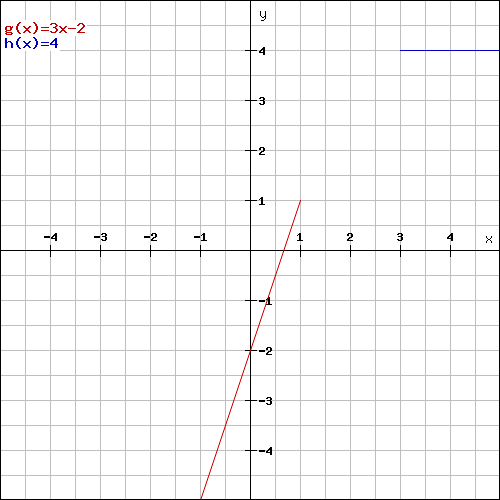
\includegraphics[width=0.5\textwidth]{image1.png}
\end{center}
Somit handelt es sich bei der gesuchten Funktion um
\begin{equation*}
\begin{split}
f(x) & = ax^3 + bx^2 + cx + d\\
f'(x) & = 3ax^2 + 2bx + c
\end{split}
\end{equation*}
mit den folgenden Bedingungen:
\begin{equation*}
\begin{split}
g(1) & = f(1)\\
h(3) & = f(3)\\
g'(1) & = f'(1)\\
h'(1) & = f'(1)
\end{split}
\end{equation*}
Daraus lässt sich folgendes Gleichungssystem aufstellen:
\begin{equation*}
\begin{split}
3\cdot 1-2 & = a\cdot 1^3 + b\cdot 1^2 + c\cdot 1 + d\\
4 & = a\cdot 3^3 + b\cdot 3^2 + c\cdot 3 + d\\
3 & = 3a\cdot 1^2 + 2b \cdot 1 + c\\
0 & = 3a\cdot 3^2 + 2b\cdot 3 + c
\end{split}
\end{equation*}
Welches sich mit dem CAS lösen lässt:
\[
solve \Vast(
\begin{cases}
1 = a + b + c + d\\
4 = a\cdot 3^3 + b\cdot 3^2 + c\cdot 3 + d\\
3 = 3a + 2b  + c\\
0 = 3a\cdot 3^2 + 2b\cdot 3 + c
\end{cases}
,\{a,b,c,d\}\Vast)
\]
Als Ergebnis erhalten wir:
\begin{equation*}
\begin{split}
a & = 0\\
b & = -0.75\\
c & = 4.5\\
d & = -2.75
\end{split}
\end{equation*}
Somit ergibt sich für $f(x)$:
$$f(x) = -0.75x^2 + 4.5x - 2.75,\ 1 \leq x \leq 3$$
Eingezeichnet in das Koordinatensystem:
\begin{center}
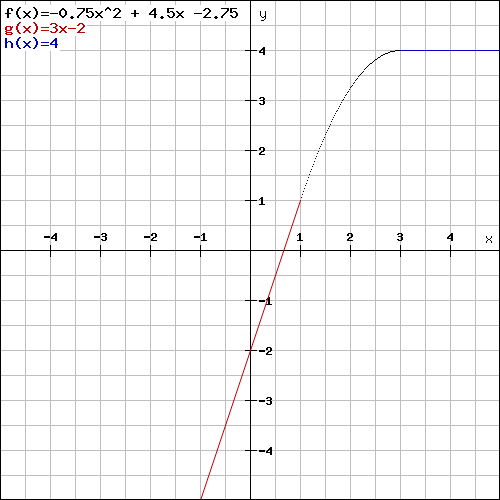
\includegraphics[width=0.75\textwidth]{image2.png}
\end{center}
\pagebreak
\section{Biegelinien}
\subsection{Wichtige Variablen}
\begin{itemize}
\item Elastizitätsmodul $E$:
	\subitem Werkstoffspezifischer Wert in $\frac{N}{m^2}$
\item Flächenträgheitsmoment $I$:
	\subitem \parbox[t]{\linewidth}{
	Formspezifischer Wert in $m^4$}
\item Streckenlast $q(x)$:
	\subitem \parbox[t]{\linewidth}{
	\begin{equation*}
	\begin{split}
	w''''(x) & = \frac{1}{E \cdot I}q(x)\\
	w''''(x) & = \frac{1}{E \cdot I} \cdot q
	\end{split}
	\end{equation*}
	in Newton pro Meter $\frac{N}{m}$}
\item Querkraft $Q(x)$:
	\subitem \parbox[t]{\linewidth}{
	\begin{equation*}
	\begin{split}
	w'''(x) & = \frac{1}{E \cdot I}-Q(x)\\
	w'''(x) & = \frac{1}{E \cdot I}\cdot (qx + c_1)
	\end{split}
	\end{equation*}
	in Newton $N$}
\item Biegemoment $w''(x)$:
	\subitem \parbox[t]{\linewidth}{
	\begin{equation*}
	\begin{split}
	w''(x) & = \frac{1}{E \cdot I}-M(x)\\
	w''(x) & = \frac{1}{E \cdot I}\cdot (\frac{1}{2} qx^2 + c_1 \cdot x + c_2)
	\end{split}
	\end{equation*}
	in Newtonmeter $Nm$}
\item Steigung der Biegelinie $w'(x)$
	\subitem $$w'(x) = \frac{1}{E \cdot I}\cdot (\frac{1}{6} qx^3 + \frac{1}{2} c_1x^2 + c_2x + c_3)$$
\item Biegelinie $w(x)$
	\subitem \parbox[t]{\linewidth}{ 
	$$w(x) = \frac{1}{E \cdot I}\cdot (\frac{1}{24} qx^4 + \frac{1}{6} c_1x^3 + \frac{1}{6} c_2x^2 + c_3x + c_4)$$
	in Meter $m$}
\end{itemize}
\begin{table}[h!]
  \begin{center}
    \caption{Ermittlung der Integrationskonstanten}
    \label{tab:table2}
    \begin{tabular}{l|c|c|c|c} % <-- Alignments: 1st column left, 2nd middle and 3rd right, with vertical lines in between
      \textbf{Art der} & \textbf{Biegung} & \textbf{Steigung} & \textbf{Moment} & \textbf{Querkraft}\\
      \textbf{Randbedingung} & $w$ & $w'$ & $w''$ & $w'''$\\
      \hline
      Festlager / Loslager & 0 & $\neq 0$ & 0 & $\neq 0$\\
      \hline
      Einspannung & 0 & 0 & $\neq 0$ & $\neq 0$\\
      \hline
      Loses Ende & $\neq 0$ & $\neq 0$ & 0 & 0\\
    \end{tabular}
  \end{center}
\end{table}
\pagebreak
\subsection{Mathematischer Ansatz \& Beispiel}
Gegeben sei ein Träger für den gilt:
\begin{equation*}
\begin{split}
E & = 200 \cdot 10^9 \frac{N}{m^2}\\
I & = \frac{1}{12}(B \cdot H^3 - b \cdot h^3)\\
B & = 0.3\\
H & = 0.5\\
b & = 0.27\\
h & = 0.47\\
q(x) & = -8000 \frac{N}{m}
\end{split}
\end{equation*}
Des Weiteren ist ein Festlager bei $x = 0$ und ein Loslager bei $x = 10$ bekannt.
Es soll überprüft werden, ob das Biegemoment eines Trägers den Betrag von $150000 Nm$ überschreitet.
Es lassen sich folgende Bedingungen aufstellen:
\begin{equation*}
\begin{split}
w(0) & = 0\\
w''(0) & = 0 \Rightarrow \frac{1}{e \cdot I} \cdot c_2 \Rightarrow \underline{\underline{c_2 = 0}}\\
w(10) & = 0\\
w''(10) & = 0 \Rightarrow 0 = \frac{1}{e \cdot I} \cdot \Bigg{(}\frac{1}{2} \cdot (-8000) \cdot 10^2 + 10 \cdot c_1\Bigg{)}\\
0 & = -400000 + 10 \cdot c_1\\
c_1 & = 40000
\end{split}
\end{equation*}
Somit ist das Biegemoment $- M(x) = - \frac{1}{2} \cdot 8000x^2 + 40000x$ bzw $M(x) = \frac{1}{2} \cdot 8000x^2 - 40000x$ bekannt.
Um die $x$-Stelle des maximale Biegemoment zu bestimmen wird $M'(x) = 0$ gesetzt.
\begin{equation*}
\begin{split}
M'(x) & = 0\\
8000x - 40000 & = 0\\
x & = 5
\end{split}
\end{equation*}
Somit ist uns bekannt, dass das maximale Biegemoment bei $x = 5$ vorliegt.
Nun berechnen wir das Biegemoment an $x = 5$.
\begin{equation*}
\begin{split}
M(5) & = 4000 \cdot 5^2 - 40000 \cdot 5\\
M(5) & = -100000
\end{split}
\end{equation*}
Somit hält der Träger, da
$$|-100000| < 150000$$
\section{Wachstumsfunktionen}


\subsection{Wachstum und Zerfall}
Generell gilt $f(t) = a \cdot c^t = a \cdot e^{k \cdot t}$ 
\subsubsection{Bestand $f(t)$}
Der Bestand ist definiert als
$$f(t) = a \cdot c^t$$
wobei $c$ definiert ist als:
$$c = e^k$$
\subsubsection{Wachstumsfaktor $c$}
\subsubsection{Wachstumskonstante $k$}
Es gilt:
$$k = \ln{(c)}$$
Bei Wachstum gilt $k > 0$ und bei Zerfall $k < 0$
\subsubsection{Verdopplungszeit}
Für die Verdopplungszeit $t_v$ gilt:
$$t_v = \frac{\ln{(2)}}{k}$$
\subsubsection{Halbierungszeit}
Für die Halbierungszeit $t_h$ gilt:
$$t_h = \frac{\ln{(0.5)}}{k}$$
\pagebreak
\subsubsection{Wachstumsgeschwindigkeit}
Die Wachstumsgeschwindigkeit zum Zeitpunkt $t$ entspricht der Ableitung der Wachstumsfunktion am Zeitpunkt $t$.
Somit gilt:
\begin{equation*}
\begin{split}
f(t) & = a \cdot e^{k \cdot t}\\
f'(t) &= k \cdot a \cdot e^{k \cdot t}
\end{split}
\end{equation*}
Also $$f'(t) = k \cdot f(t)$$
\section{$e$ - Funktionen}
Die Ableitung von $e^x$ bleibt $e^x$.\\
Hat man also $f(x) = e^{2x}$, wird zu erst der Exponen betrachtet, als $2 \cdot x$, was sich zu $2$ ableitet.\\
Diese $2$ ist wird jetzt vor das $e$ geschrieben, sodass sich für die Ableitung von $f(x) = e^{2x}$ $f'(x) = 2 \cdot e^{2x}$ ergibt.\\
Es folgen einige Beispiele:\\
\begin{equation*}
\begin{split}
f(x) & = a \cdot e^{\frac{1}{a} \cdot x^2}\\
f'(x) & = 2x \cdot e^{\frac{1}{a} \cdot x^2}
\end{split}
\end{equation*}
Der Faktor $a$ kürzt sich mit der Ableitung $\frac{2x}{a}$ des Exponenten weg.
\begin{equation*}
\begin{split}
f(x) & = e^{2x^2-3x}\\
f'(x) & = 4x - 3 \cdot e^{2x^2-3x}
\end{split}
\end{equation*}
da die Ableitung des Exponenten zum Faktor für die Basis, also $e^{...}$ wird.\\
Bezüglich Logarithmen gilt:$$\ln{(e^{2x})} = 2x$$
\pagebreak
\part{VEKTOREN}
\section{Ortsvektoren}
Der Ortsvektor eines Punktes $P$ geht vom Ursprung $O$ nach $P$. Somit gilt $\vec{p} = \vec{OP}$.
\section{Addition und Subtraktion}
Es gilt:
$$\vec{a} - \vec{b} = \begin{pmatrix}a_x\\a_y\\a_z\end{pmatrix} - \begin{pmatrix}b_x\\b_y\\b_z\end{pmatrix} = \begin{pmatrix}a_x - b_x\\a_y - b_y\\a_z - b_z\end{pmatrix}$$
\section{Multiplikation}
\subsection{Multiplikation mit einem Skalar}
Wird ein Vektor $\vec{v}$ mit einem Skalar $r$ multipliziert, so wird jedes Element des Vektors mit dem Skalar multipliziert.\\
Es gilt:
$$r \cdot \vec{v} = \begin{pmatrix}r \cdot v_x\\r \cdot v_y\\r \cdot v_z\end{pmatrix}$$
\subsection{Skalarprodukt}
Werden zwei Vektoren multipliziert, so erhält man einen Skalar.\\
Es gilt:
$$\vec{a} \cdot \vec{b} = a_x \cdot b_x + a_y \cdot b_y + a_z \cdot b_z$$
\section{Betrag (Länge) eines Vektors}
Es gilt:
$$|\vec{a}| = \sqrt{a_{x}^{2} + a_{y}^{2} + a_{z}^{2}}$$
\section{Vektor durch zwei Punkte}
Der Vektor $\vec{AB}$ zwischen Punkt $A$ und $B$ lässt sich mit den Ortsvektoren $\vec{a}$ und $\vec{b}$ berechnen.\\
Es gilt:
$$\vec{AB} = \vec{b} - \vec{a}$$
\section{Orthogonalitätsbedingung}
Wenn $\vec{a}\ \bot\ \vec{b}$, dann gilt:
$$\vec{a} \cdot \vec{b} = 0$$
also
$$a_x \cdot b_x + a_y \cdot b_y + a_z \cdot b_z = 0$$
\section{Winkel zwischen zwei Vektoren}
Der Winkel $\alpha$ zwischen den Vektoren $\vec{a}$ und $\vec{b}$ lässt sich wie folgt berechnen:
\subsection{Mathematischer Ansatz}
$$\alpha = \arccos{\frac{\vec{a} \cdot \vec{b}}{|\vec{a}| \cdot |\vec{b}|}}$$
\subsection{CAS}
$$arccos(\frac{dotP(a, b)}{norm(a) \cdot norm(b)})$$
\pagebreak
\section{Abstand windschiefer Geraden}
\subsection{Mathematischer Ansatz}
Der Abstand zweier Geraden $g : \vec{x} = \vec{a} + r \cdot \vec{b}$ und $h : \vec{x} = \vec{v} + s \cdot \vec{w}$, wobei die Faktoren $r$ und $s$ unbekannt sind, lässt sich mit Hilfe des Vektorzuges ermitteln.\\
Für den Vektorzug $\vec{d}$, welcher einen Vektor zwischen den Geraden $g$ und $h$ bildet gilt:
$$\vec{d} = g - h$$
also:
$$\vec{d} = (\vec{a} + r \cdot \vec{b}) - (\vec{v} + s \cdot \vec{w})$$
Des Weiteren müssen die Richtungsvektoren $\vec{b}$ und $\vec{w}$ orthogonal zu $\vec{d}$ sein.\\
Es gilt also:
$$\vec{b} \cdot \vec{d} = 0$$
$$\vec{w} \cdot \vec{d} = 0$$
Somit lassen sich die 2 Gleichungen nach den beiden Unbekannten $r$ und $s$ auflösen.
$r$ und $s$ werden nun in $\vec{d}$ eingesetzt und $|\vec{d}|$ kann berechnet werden:
$$|\vec{d}| = \sqrt{d_{x}^{2} + d_{y}^{2} + d_{z}^{2}}$$
\subsection{CAS}
$solve(dotP(d,b) = 0,r)$, das Ergebnis für $r$ einsetzen und\\
$solve(dotP(d,w) = 0,s)$.\\
Beides in $d$ einsetzen.\\
$norm(d) \rightarrow$ done.
\pagebreak
\section{Kreuzprodukt und Normalenvektor}
Der Normalenvektor $\vec{n}$ steht senkrecht auf der Ebene $E$.\\
Wobei der Betrag $|\vec{n}|$ des Normalenvektors der Fläche der Ebene entspricht.\\
Er lässt sich aus dem Kreuzprodukt der beiden Spannvektoren von $E$ berechnen. Somit gilt:
$$\vec{n} = \vec{a} \times \vec{b} = \begin{pmatrix}a_y \cdot b_z - a_z \cdot b_y\\a_z \cdot b_x - a_x \cdot b_z\\a_x \cdot b_y - a_y \cdot b_x\end{pmatrix}$$
Des Weiteren lässt sich des Kreuzprodukt mit der \textit{Zuhalteregel} ($\rightarrow$ Internet) von Hand berechnen oder mit dem CAS:\\
$$crossP(a,b)$$
\section{Ebenen}
\subsection{Parameterform}
Die Parameterform definiert eine Ebene $E$ mit drei Punkten $A$, $B$ und $C$ als:
$$E : \vec{x} = \vec{OA} + r \cdot \vec{AB} + s \cdot \vec{AC}$$
wobei $\vec{x}$ als Abtastvektor, $\vec{OA}$ als Hinführungsvektor und $\vec{AB}$, sowie $\vec{AC}$ als Spannvektoren bezeichnet werden.
\subsection{Normalenform}
Die Normalenform definiert eine Ebene $E$ mit einem Hinführungsvektor $\vec{p}$ und dem Normalenvektor $\vec{n}$ als:
$$E : (\vec{x} - \vec{p}) \cdot \vec{n} = 0$$
\subsection{Koordinatenform}
Die Koordinatenform entspricht der ausmultiplizierten Normalenform.\\
Es gilt:
$$x \cdot x_n + y \cdot y_n + z \cdot z_n = d$$
wobei $d$ dem Skalarprodukt $\vec{p} \cdot \vec{n}$ aus der Normalenform entspricht.
\subsection{Achsenabschnittsform}
Die Achsenabschnittsform entspricht der durch $d$ dividierten Koordinatenform.
$$\frac{1}{\frac{d}{x_n}} \cdot x + \frac{1}{\frac{d}{y_n}} \cdot y + \frac{1}{\frac{d}{z_n}} \cdot z = 1$$
was als 
$$\frac{1}{x_s} \cdot x + \frac{1}{y_s} \cdot y + \frac{1}{z_s} \cdot z = 1$$
zusammengefasst werden kann.
\subsection{Umformen von Ebenengleichungen}
\subsubsection{Koordinatenform in Parameterform}
Gegeben ist die Ebenengleichung $E : a \cdot x + b \cdot y + c \cdot z = d$, die in die Parameterform umgewandelt werden soll.\\
Dazu wird zu erst durch Umformen der Gleichung eine Unbekannte eliminiert (z.B. $x = -\frac{b \cdot y}{a} - \frac{c \cdot z}{a} + \frac{d}{a}$).\\
Da die Parameterform aus Vektoren besateht, schreiben wir die drei Gleichungen für die $x$, $y$ und $z$ Koordinaten untereinander:\\
\begin{equation*}
\begin{split}
x & = -\frac{b}{a} \cdot y - \frac{c}{a} \cdot z + \frac{1}{a} \cdot d\\
y & = \ \ \ 1 \cdot y + 0\ \cdot z + 0 \cdot d\\
z & = \ \ \ 0 \cdot y + 1\ \cdot z + 0 \cdot d\\
\end{split}
\end{equation*}
Als Vektor ergibt sich somit:
$$\begin{pmatrix}x\\y\\z\end{pmatrix} = \begin{pmatrix}-\frac{b}{a} \cdot y\\\ \ 1 \cdot y\\\ \ 0 \cdot y\end{pmatrix} + \begin{pmatrix}- \frac{c}{a}\cdot z\\\ \ 0 \cdot z\\\ \ 1 \cdot z\end{pmatrix} + \begin{pmatrix}\frac{1}{a} \cdot d\\0 \cdot d\\0 \cdot d\end{pmatrix}$$
Ausmultipliziert:
$$\vec{x} = \begin{pmatrix}\frac{1}{a} \cdot d\\0\\0\end{pmatrix} + y \cdot \begin{pmatrix}-\frac{b}{a}\\1\\0\end{pmatrix} + z \cdot \begin{pmatrix}- \frac{c}{a}\\0\\1\end{pmatrix}$$ 
\pagebreak
\subsubsection{Parameterform in Normalenform}
Gegeben ist die Ebenengleichung $E : \vec{x} = \vec{p} + r \cdot \vec{a} + s \cdot \vec{b}$, die in die Normalenform umgewandelt werden soll.\\
Dies wird durch die Berechnung des Kreuzproduktes ermöglicht:\\
$$E : (\vec{x} - \vec{p}) \cdot (\vec{a} \times \vec{b}) = 0$$
\section{Lagebeziehung zwischen Gerade und Ebene}
\textit{$\rightarrow$ Seite 260}\\
Gegeben ist eine Gerade $g : \vec{x} = \vec{u} + t \cdot \vec{v}$ und eine\\
Ebene $E : \vec{x} = \vec{a} + r \cdot \vec{b} + s \cdot \vec{c}$. Im Folgenden soll die Lagebeziehung von $g$ und $E$ überprüft werden. 
\subsection{1. Fall: Parallel}
Um unnötige Rechnungen zu ersparen wird zu erst getestet, ob $g \parallel E$.\\
Wenn $g \parallel E$ ist, dann ist $g\ \bot\ \vec{n}$, dem Normalenvektor der Ebene.\\
Somit muss überprüft werden, ob $\vec{v} \cdot (\vec{b} \times \vec{c}) = 0$.
\subsection{2. Fall: Schnittpunkt}
\subsubsection*{1. Variante}
Wenn es einen Schnittpunkt gibt, gilt $g = E$, also:
$$\vec{u} + t \cdot \vec{v} = \vec{a} + r \cdot \vec{b} + s \cdot \vec{c}$$
Nun werden die einzelnen $x$, $y$ und $z$ Werte betrachtet:
$$\begin{pmatrix}u_x\\u_y\\u_z\end{pmatrix} + t \cdot \begin{pmatrix}v_x\\v_y\\v_z\end{pmatrix} = \begin{pmatrix}a_x\\a_y\\a_z\end{pmatrix} + r \cdot \begin{pmatrix}b_x\\b_y\\b_z\end{pmatrix} + s \cdot \begin{pmatrix}c_x\\c_y\\c_z\end{pmatrix}$$
woraus sich drei Gleichungen und drei Unbekannte ergeben:
\begin{equation}
\begin{split}
u_x + t \cdot v_x & = a_x + r \cdot b_x + s \cdot c_x\\ 
u_y + t \cdot v_y & = a_y + r \cdot b_y + s \cdot c_y\\ 
u_z + t \cdot v_z & = a_z + r \cdot b_z + s \cdot c_z
\end{split}
\end{equation}
Nachdem nach $t$, $r$ und $s$ aufgelöst wurde, lässt sich $t$ in $g$ oder $r$ und $s$ in $E$ einsetzen und es ergibt sich $\vec{s}$, beziehungsweise daraus folgend der
Schnittpunkt $S$.
\subsubsection*{2. Variante}
$E$ wird in Koordinatenform umgewandelt. Dazu wird zuerst der Normalenvektor von $E$ berechnet:
$$\vec{n} = \vec{b} \times \vec{c}$$
Außerdem muss $d$ berechnet werden:
$$d = \vec{n} \cdot \vec{a}$$
Daraus ergibt sich die Koordinatenform der Ebene:
$$x \cdot n_x + y \cdot n_y + z \cdot n_z = d$$
Nun wird $g$ in die $x$, $y$ und $z$ Komponenten unterteilt.\\
Es ergeben sich die drei Gleichungen:
\begin{equation*}
\begin{split}
x & = u_x + t \cdot v_x\\
y & = u_y + t \cdot v_y\\
z & = u_z + t \cdot v_z
\end{split}
\end{equation*}
welche nun in $E$ eingesetzt werden:
$$(u_x + t \cdot v_x) \cdot n_x + (u_y + t \cdot v_y) \cdot n_y + (u_z + t \cdot v_z) \cdot n_z = d$$
Nun wird nach $t$ aufgelöst und in $g$ eingesetzt. $g$ lässt sich anschließend als $\vec{s}$ ausmultiplizierten, was dem Schnittpunkt $S$ entspricht.
\subsection{3. Fall: Identisch}
Falls $g \in E$, so ergibt sich beim Berechnen des Schnittpunktes eine wahre Aussage.\\
Des Weiteren gilt $g \parallel E$, also $\vec{v} \cdot (\vec{b} \times \vec{c}) = 0$.
\subsection{CAS}
Das Gleichungssystem oben (1) lässt sich mit dem CAS wie folgt lösen:\\
\textit{menu} $\rightarrow$ \textit{3 : Algebra} $\rightarrow$ \textit{7 : Solve System of Equations} $\rightarrow$ \textit{1 : Solve System of Equations...}\\
Falls der CAS:
\begin{itemize}
\item eine Lösung findet, existiert ein Schnittpunkt.
\item \textit{false} zurückgibt, sind sie Parallel.
\item \textit{true} zurückgibt, ist $g \in E$.
\end{itemize}
\section{Lagebeziehung zwischen Punkt und Ebene}
Ähnlich wie bei der Lagebeziehung zwischen Gerade und Ebene, wird der Punkt $P$ in einen Vektor $\vec{p}$ umgewandelt und der Ebene $E$ gleichgesetzt.\\
Somit ergibt sich:
$$\begin{pmatrix}p_x\\p_y\\p_z\end{pmatrix} = \begin{pmatrix}a_x\\a_y\\a_z\end{pmatrix} + r \cdot \begin{pmatrix}b_x\\b_y\\b_z\end{pmatrix} + s \cdot \begin{pmatrix}c_x\\c_y\\c_z\end{pmatrix}$$
woraus sich 3 Gleichungen und 2 Unbekannte ergeben:
\begin{equation*}
\begin{split}
p_x & = a_x + r \cdot b_x + s \cdot c_x\\ 
p_y & = a_y + r \cdot b_y + s \cdot c_y\\ 
p_z & = a_z + r \cdot b_z + s \cdot c_z
\end{split}
\end{equation*}
Falls $P \in E$, dann lassen sich $r$ und $s$ berechnen.\\
Falls $P \notin E$, so ergibt sich eine widersprüchliche Aussage.
\subsection{CAS}
Falls der CAS:
\begin{itemize}
\item eine Lösung findet, gilt $P \in E$.
\item keine Lösung findet, gilt $P \notin E$.
\end{itemize}
\section{Winkel zwischen Gerade und Ebene}
Der Winkel zwischen dem Richtungsvektor $\vec{v}$ einer Gerade $g$ und einer Ebene $E$ wird mit Hilfe des Normalenvektors $\vec{n}$ der Ebene berechnet.
Für den Winkel $\alpha$ zwischen $g$ und $E$ gilt:
$$\alpha = 90 - \arccos{\frac{\vec{v} \cdot \vec{n}}{|\vec{v}| \cdot |\vec{n}|}}$$
\pagebreak
\section{Flächenberechnung von Ebenen}
\subsection{Fläche eines Parallelogramms}
Fläche eines Parallelogramms entspricht dem Betrag des Normalenvektors der Ebene.\\
Somit gilt:
$$A_{\Parallelogramm} = |\vec{n}|$$
beziehungsweise
$$A_{\Parallelogramm} = |\vec{a}| \cdot |\vec{b}| \cdot \sin{\alpha}$$
\subsection{Fläche eines Quadrates}
Bei einem Quadrat kann diese Formel zu
$$A_{\square} = |\vec{a}| \cdot |\vec{b}|$$
vereinfacht werden, da $\vec{a}\ \bot\ \vec{b}$, weshalb $\alpha = 90\degree$, sodass $\sin{\alpha} = 1$.
\subsection{Fläche eines Dreiecks}
Da ein Dreieck der halben Fläche eines Parallelogramms entspricht gilt:
$$A_{\triangle} = \frac{|\vec{n}|}{2}$$
beziehungsweise
$$A_{\triangle} = \frac{|\vec{a}| \cdot |\vec{b}| \cdot \sin{\alpha}}{2}$$
\subsection{Fläche eines beliebigen Vierecks}
Um die Fläche iens beliebigen Vierecks zu berechnen, wir das Viereck in Dreiecke unterteilt, welche wie gewöhlich berechnet und letztendlich aufsummiert werden.\\
Für ein Viereck mit den Punkten $A$, $B$, $C$ und $D$ gilt:
$$A = \frac{|\vec{AB} \times \vec{AC}|}{2} + \frac{|\vec{AC} \times \vec{AD}|}{2}$$
\section{Schnittpunkte von Ebene und Koordinatenachsen}
Gegeben sei eine Ebene mit der Ebenengleichung in Koordinatenform:\\
$$E : a \cdot x + b \cdot y + c \cdot z = d$$
Um den Schnittpunkt $S_x$ mit der X-Achse zu errechnen, wird $y = 0$ und $z = 0$ gesetzt, sodass
$$a \cdot x = d$$
überbleibt und nach $x$ umgeformt werden kann. Selbiges gilt zum Berechnen von $S_y$ und $S_z$.
\section{Schnittgerade zwischen zwei Ebenen}
Gegeben sind zwei Ebenengelichungen in...
\subsection{Parameterform}
$$E_1 : \vec{x} = \vec{a} + q \cdot \vec{b} + r \cdot \vec{c}$$
$$E_2 : \vec{x} = \vec{u} + s \cdot \vec{v} + t \cdot \vec{w}$$
Für die Schnittgerade $g$ gilt $E_1 = E_2$, also:
$$\begin{pmatrix}a_{x}\\a_{y}\\a_{z}\end{pmatrix} + q \cdot \begin{pmatrix}b_{x}\\b_{y}\\b_{z}\end{pmatrix} + r \cdot \begin{pmatrix}c_{x}\\c_{y}\\c_{z}\end{pmatrix} = \begin{pmatrix}u_{x}\\u_{y}\\u_{z}\end{pmatrix} + s \cdot \begin{pmatrix}v_{x}\\v_{y}\\v_{z}\end{pmatrix} + t \cdot \begin{pmatrix}w_{x}\\w_{y}\\w_{z}\end{pmatrix}$$
woraus sich drei Gleichungen und vier Unbekannte ergeben:
\begin{equation}
\begin{split}
a_x + q \cdot b_x + r \cdot c_x & = u_x + s \cdot v_x + t \cdot w_x\\
a_y + q \cdot b_y + r \cdot c_y & = u_y + s \cdot v_y + t \cdot w_y\\
a_z + q \cdot b_z + r \cdot c_z & = u_z + s \cdot v_z + t \cdot w_z
\end{split}
\end{equation}
Dieses Gleichungssystem lässt sich zu einer Geradengleichung $g$ auflösen, sodass sich für
$$g : \vec{x} = \vec{n} + s \cdot \vec{m}$$
ergibt.
\subsubsection{CAS}
Das Gleichungssystem oben (2) lässt sich mit dem CAS wie folgt lösen:\\
\textit{menu} $\rightarrow$ \textit{3 : Algebra} $\rightarrow$ \textit{7 : Solve System of Equations} $\rightarrow$ \textit{1 : Solve System of Equations...}
\subsection{Koordinatenform}
$$E_1 : a \cdot x + b \cdot y + c \cdot z = d$$
$$E_2 : t \cdot x + u \cdot y + v \cdot z = w$$
Dadurch ergeben sich zwei Gleichungen und drei Unbekannte, die sich nur teilweise auflösen lassen.\\
Zum Beispiel:
\begin{equation*}
\begin{split}
x & = y + i\\
y & = y\\
z & = j
\end{split}
\end{equation*}
wobei $i$ und $j$ sich durch Auflösen des Gleichungssystems ergeben.\\
Dadurch ergibt sich für $g$:
\begin{equation*}
\begin{split}
g : \vec{x} & = \begin{pmatrix}y + i\\y\ \ \ \ \ \\\ \ \ \ \ j\end{pmatrix}\\
g : \vec{x} & = \begin{pmatrix}y\\y\\0\end{pmatrix} + \begin{pmatrix}i\\0\\j\end{pmatrix}\\
g : \vec{x} & = \begin{pmatrix}1\\1\\0\end{pmatrix} \cdot y + \begin{pmatrix}i\\0\\j\end{pmatrix}
\end{split}
\end{equation*}
wobei durch das Ausklammern von $y$ der Richtungsvektor entsteht.
\pagebreak
\section{Winkel zwischen zwei Ebenen}
Um den Schnittwinkel zweier Ebenen $E_1$ und $E_2$ zu berechnen wird der Winkel der Normalenvektoren $\vec{n_1}$ und $\vec{n_2}$ berechnet.\\
$\rightarrow$ Siehe \textit{Winkel zwischen zwei Vektoren}
\section{Spatvolumen}
Gegeben seien die Vektoren $\vec{a}$, $\vec{b}$ und $\vec{c}$. Es soll das Volumen mit der Grundfläche eines Parallelogramms berechnet werden, welches sich zwischen diesen Vektoren bildet.\\
Für das Volumen gilt: $V = h \cdot A$, wobei $A = |\vec{a} \times \vec{b}|$. $h$ ergibt sich aus dem Skalarprodukt von $\cos{\varphi}$ und $\vec{c}$. Also $h = \cos{\varphi} \cdot \vec{c}$, wobei 
für $\cos{\varphi}$ gilt: $\cos{\varphi} = \frac{\vec{n} \cdot \vec{c}}{|\vec{n}| \cdot |\vec{c}|}$.\\
Somit ergibt sich:
$$V = \frac{(\vec{a} \times \vec{b}) \cdot \vec{c}}{(|\vec{a} \times \vec{b}|) \cdot |\vec{c}|} \cdot |\vec{c}| \cdot |\vec{a} \times \vec{b}|$$
Vereinfacht:
$$V = (\vec{a} \times \vec{b}) \cdot \vec{c}$$
\subsection{Grundfläche entspricht Parallelogramm}
$$V = (\vec{a} \times \vec{b}) \cdot \vec{c}$$
\subsection{Volumen einer Pyramide}
$$V = \frac{1}{3} \cdot (\vec{a} \times \vec{b}) \cdot \vec{c}$$
\subsection{Volumen eines Tetraeders}
(Pyramide mit $\triangle$ als Grundfläche)
$$V = \frac{1}{6} \cdot (\vec{a} \times \vec{b}) \cdot \vec{c}$$
\pagebreak
\section{CAS Commands}
\subsection{dotP}
Zur Berechnung des Skalarproduktes zweier Vektoren $\vec{a}$ und $\vec{b}$.\\
CAS:\\
$$dotP(a,b)$$
\subsection{norm}
Zur Berechnung des Betrags eines Vektors $|\vec{v}|$.\\
CAS:\\
$$norm(v)$$
\subsection{crossP}
Zur Berechnung des Kreuzproduktes $\vec{a} \times \vec{b}$ zweier Vektoren.\\
CAS:\\
$$crossP(a,b)$$
\pagebreak
\part{STOCHASTIK}
\subsection{Definitionen}
\begin{itemize}
\item Statistische Erhebungen
	\subitem \parbox[t]{\linewidth}{
	Die Durchführung einer Statistik\\
    (z.B. das Befrage von Personen / Zählen von Gegenständen)\\
	}
\item Merkmalsträger
	\subitem \parbox[t]{\linewidth}{
	Das untersuchte Objekt der Statistik\\
    (z.B. Personen oder Autos)
	}
\item Merkmal
	\subitem \parbox[t]{\linewidth}{
	Der im Zusammenhang mit dem Merkmalsträger untersuchte Wert\\
    (z.B. Größe oder Geschwindigkeit)
	}
\item Grundgesamtheit
	\subitem \parbox[t]{\linewidth}{
	Die Summe aller Merkmalsträger
	}
\item Stichprobe
	\subitem \parbox[t]{\linewidth}{
	ausgewählte Merkmalsträger der Grundgesamtheit
	}
\item Stichprobenumfang
	\subitem \parbox[t]{\linewidth}{
	Die Anzahl $n$ der Merkmalsträger einer Stichprobe
	}
\item Urliste
	\subitem \parbox[t]{\linewidth}{
	Die Beobachtugsliste (Datentabelle)
	}
\item Stichprobenwert
	\subitem \parbox[t]{\linewidth}{
	Ein Tabelleneintrag (eine Zeile)
	}
\item Qualitative Merkmale
	\subitem \parbox[t]{\linewidth}{
	nominal- oder Ordinalskala
	}
\item Quantitative Merkmale
	\subitem \parbox[t]{\linewidth}{
	Messbar mit Zahlenwerten (metrisch)\\
    - diskret: $n \in \mathbb{Z}$\\
    - stetig: $n \in \mathbb{R}$
	}
\item Absolute Häufigkeit $H(ai)$
	\subitem \parbox[t]{\linewidth}{
	bei $n$ Stichprobenwerten tritt ein Merkmal $H$-mal auf
	}
\item Relative Häufigkeit $h(ai)$
	\subitem \parbox[t]{\linewidth}{
	das Merkmal tritt in H/n aller Fälle auf (Bruch bzw \%)
	}
\item Häufigkeitstabelle / Häufigkeitsverteilung
	\subitem \parbox[t]{\linewidth}{
	Tabelle mit H und Merkmalen
	}
\item Klasseneinteilung
	\subitem \parbox[t]{\linewidth}{
	Einteilen von Intervallen in Teilintervalle (zur Reduzierung der Datenmenge)\\
    z.B Werte 10 - 20, Werte 20 - 30, etc
	}
\item Histogramm
	\subitem \parbox[t]{\linewidth}{
	Diagramm, welches die Unterschiede verschiedener Klassen darstellt
	}
\item Häufigkeitspolygon
	\subitem \parbox[t]{\linewidth}{
	Der Graph der durch Verbinden der Histogramm-Werte entsteht
	}
\item Summenpolygon
	\subitem \parbox[t]{\linewidth}{
	Die Summe der Histogramm werte dargestellt als Funktion
	}
\item Spannweite $R$
	\subitem \parbox[t]{\linewidth}{
	Die Differenz zwischen dem größten Stichprobenwert $X_{max}$ und dem kleinsten $X_{min}$
	}
\item Standardabweichung $\sigma x$
	\subitem \parbox[t]{\linewidth}{
	Durchschnittliche Abweichungen vom Mittelwert
	}
\end{itemize}
\pagebreak
\section{REGRESSION}
\subsection{Korrelation r}
Die Korrelation $r$ ist ein Maß für die Güte der Regression,
also ein Maß für die Stärke des funktionalen Zusammenhangs.
\begin{equation}
\begin{split}
ges.: g(x) & = mx\\
s & = (\Delta y_1)^2 + (\Delta y_2)^2 + (\Delta y_3)^2 ...\\
s(m) & = (y_1 - mx_1)^2 + (y_2 - mx_2)^2 + (y_3 - mx_3)^2 + ...\\
s'(m) & = 0\\
r^2 & = mx \cdot my\\
\end{split}
\end{equation}
(3) Berechnung der Abstände ohne Hilfsmittel
\subsection{Aufgaben zur Regression}
\subsubsection{Aufgabe 3}
Eine der drei Geraden $g$ mit $g(x) = 0.2x + 1.5$, $h$ mit $h(x) = 0.4x + 0.8$
und $i$ mit $i(x) = 0.5x + 0.5$ ist eine Regressionsgerade zu den Datenpaaren (0|1), 
(2|2), (4|1) und (6|4).\\
Entscheiden Sie ohne Verwendung des Regressionsbefehls des Rechners, welche. Dokumentieren
Sie einen Lösungsweg, der auch ohne GTR oder CAS\\
nachvollziehbar ist.\\
\\
\textbf{Rechnung}:\\
\begin{equation*}
\begin{split}
geg.: i(x) & = 0.5x + 0.5\\
ges.: s\ \ \ \ &\\
s & = (\Delta y_1)^2 + (\Delta y_2)^2 + (\Delta y_3)^2 ...\\
s(m) & = (y_1 - mx_1)^2 + (y_2 - mx_2)^2 + (y_3 - mx_3)^2 + (y_4 - mx4)^2\\
s(0.5) & = (1 - (0.5 \cdot 0 + 0.5))^2 + (2 - (0.5 \cdot 2 + 0.5))^2 + (1 - (0.5 \cdot 4 + 0.5))^2 + \\
&\ \ \ \ (4 - (0.5 \cdot 6 + 0.5))^2\\
s(0.5) & = 3\\
\end{split}
\end{equation*}
\pagebreak
\subsubsection{Nicht-lineare Regression}
In einen Behälter wird fortlaufend 20 Liter Flüssigkeit eingefüllt und dann jeweils die Füllhöhe $h$ gemessen.\\
\\
a.)\\
Durch welche ganzrationale Funktion lässt sich der funktionale Zusammenhang uwischen der Füllhöhe $h$ und dem Volumen $V$
am besten beschreiben? Vergleichen Sie Modellierungen mit ganzrationalen Funktionen 2., 3. und 4. Grades miteinander.\\\\
\begin{equation*}
\begin{split}
f1(x) & = 0.000868x^2 + 1.5x -12.63\\
f2(x) & = -0.000132x^3+0.028x^2+0.0095x-1.06\\
f3(x) & = 8.7 \cdot 10^{-7} x^4-0.000373x^3 + 0.0489x^2 - 0.4753x + 0.105\\
r1^2 & = 0.981144\\
r2^2 & = 0.999137\\
r3^2 & = 0.9999\\
\end{split}
\end{equation*}
(3) Somit ist die Regression 4. Grades am besten geeignet auf Grund der genausten Korrelation 
\pagebreak
\section{WAHRSCHEINLICHKEITEN}
\subsection{Definitionen}
\subsubsection{Ergebnismenge $S$}
Die Menge aller möglichen Ergebnisse.
\subsubsection{Laplace-Versuche}
Alle Ergebnisse haben die selbe Chance aufzutreten.
\subsubsection{Nicht-Laplace-Versuche}
Alle Ergebnisse haben nicht die selbe Chance aufzutreten.
\subsubsection{Wahrscheinlichkeit $P$}
Gibt an, welche relative Häufigkeit bei häufiger Versuchsdurchführung zu erwarten ist.
\subsubsection{Ereignis}
Eine Teilmenge der Ergebnismenge $S$ mit spezifischen Eigenschaften.
\subsubsection{unmögliches Ereignis}
$P = 0 \%$ 
\subsubsection{sicheres Ereignis}
$P = 100 \%$ 
\pagebreak
\subsubsection{Inverses Baumdiagramm}
Die Pfade in umgekehrter reihenfolge (bei unterschiedlichen Verzweigungen (zb (j,n) und (m,w)))\\
Bedingte Wahrscheinlichkeit:\\
$P_A(B) = \frac{P(A \cap B)}{P(A)}$\\
Totale Wahrscheinlichkeit:\\
$P(B) = P(A \cap B) + P(\overline{A} \cap B) = P(A) \cdot P_A(B) + P(\overline{A} \cdot P_{\overline{A}}(B))$\\
\textbf{Satz von Bayes}\\
\begin{equation*}
\begin{split}
P_B(A) & = \frac{P(B \cap A)}{P(B)} = \frac{P(A \cap B)}{P(B)}\\
\ \ \ \ \ & = \frac{P(A) \cdot P(B)}{P(A) \cdot P_A(B) + P(\overline{A}) \cdot P_{\overline{A}}(B)}
\end{split}
\end{equation*}
\subsubsection{Totale Wahrscheinlichkeit}
$P(x)$ die Gesamtwahrscheinlichkeit für ein Ereignis $x$
\subsubsection{Bedingte Wahrscheinlichkeit / Häufigkeit}
Die zweite Bedingung in einem Baumdiagramm (Zweite Verzweigung)\\
$P_{ersteBedingung}(zweiteBedingung)$\\
zb $P_A(B)$
\subsection{Beispiele}
\begin{table}[h!]
  \begin{center}
    \caption{Eine 6 würfeln}
    \label{tab:table1}
    \begin{tabular}{l|c|c|c} % <-- Alignments: 1st column left, 2nd middle and 3rd right, with vertical lines in between
      \textbf{Anzahl Würfe} & \textbf{10} & \textbf{100} & \textbf{1000}\\
      \hline
      Anzahl Werte (Absolute Häufigkeit) & 4 & 16 & 163\\
      \hline
      \%-Angabe (Relative Häufigkeit) & 40\% & 16\% & 16.3\%\\
      \hline
      Richtwert (Wahrscheinlichkeit) & $\frac{1}{6}$ & $\frac{1}{6}$ & $\frac{1}{6}$\\
    \end{tabular}
  \end{center}
\end{table}
\pagebreak
\subsubsection*{Würfelspiel}
2 Würfel, gewonnen "Pasch"\\
$S = \Big\{(1,1),(1,2),(1,3),...,(3,6)\Big\}$\\
$E = \Big\{(1,1),(2,2),(3,3),(4,4),(5,5),(6,6)\Big\}$\\
\begin{table}[h!]
  \begin{center}
    \caption{Beispiele für Zufallsversuche}
    \label{tab:table1}
    \begin{tabular}{l|l} % <-- Alignments: 1st column left, 2nd middle and 3rd right, with vertical lines in between
      \textbf{Zufallversuch} & \textbf{Ergebnismenge}\\
      \hline
      Wurf einer Münze & $S = \{K,Z\}$\\
      \hline
      Random Int von 1 bis 49 & $S = \{1,2,3,...,49\}$\\
      \hline
      Körpergröße eines Säuglings & $S = \{...,46,...,55,...\}$\\
      \hline
      Ausgang eines Fußballspiels & $S = \{1,0,2\}$
    \end{tabular}
  \end{center}
\end{table}
\subsubsection*{Seite 337 Nummer 7}
Aus einer Klasse mit 18 Mädchen und 9 Jungen sollen einige Jugendliche ausgelost werden. Dies geschieht mit Hilfe eines Glückrads mit 27 gleich großen Sektoren.\\
Wie groß ist die Wahrscheinlichkeit für ein "repräsentatives" Ereignis? Welche Ereignisse wären nicht "repräsentativ"?\\
Bestimmen Sie die Wahrscheinlichkeiten für das Ergebnis\\
$(1)$ zwei Mädchen und ein Junge\\
$(2)$ vier Mädchen und zwei Jungen\\
$(3)$ sechs Mädchen und drei Jungen\\\\
Repräsentativ:\ $\frac{2}{3}$ Mädchen, $\frac{1}{3}$ Jungen\\
Nicht-Repräsentativ:\ $\frac{2}{3}$ Jungen, $\frac{1}{3}$ Mädchen\\
1: $P\ =\ (\frac{2}{3})^2 \cdot (\frac{1}{3})\ =\ 14.8\%$\\
2: $P\ =\ (\frac{2}{3})^4 \cdot (\frac{1}{3})^2\ =\ 2.19\%$\\
3: $P\ =\ (\frac{2}{3})^6 \cdot (\frac{1}{3})^3\ =\ 0.325\%$\\
\subsubsection*{Additionssatz}
Eine Kugellagerfabrik prüft Kugeln auf Abweichungen in Härte und Durchmesser.\\
Bestimme die Häufigkeit der nicht einwandfreien Kugeln. 
\begin{equation*}
\begin{split}
P(d \cup h) & = P(d) + P(h) - P(d \cap h)\\
P(d \cup h) & = \frac{65}{1000} + \frac{78}{1000} - \frac{43}{1000}\\
P(d \cup h) & = \frac{1}{10}\\
P(d \cup h) & = 10 \%\\
\end{split}
\end{equation*}
\subsubsection*{Strickwaren 2. Wahl}
\begin{equation*}
\begin{split}
P(F_a \cup M_u \cup M_a) & = P(F_a) + P(M_u) + P(M_a) - P(F_a \cap M_u) - P(F_a \cap M_a) - P(M_u \cap M_a) + \\
&\ \ \ \ P(F_a \cap M_u \cap M_a)\\
P(F_a \cup M_u \cup M_a) & = 5.1 \% + 5.3 \% + 4.7 \% - 0.4 \% - 0.9 \% - 1.5 \% + 0.3 \% \\
P(F_a \cup M_u \cup M_a) & = 12.6 \% \\
\end{split}
\end{equation*}
\subsubsection*{Schulhefte}
Kariert mit und ohne Rand und nicht Kariert\\
\begin{table}[h!]
  \begin{center}
    \caption{Werte}
    \label{tab:table1}
    \begin{tabular}{c|c|c|c} % <-- Alignments: 1st column left, 2nd middle and 3rd right, with vertical lines in between
      \textbf{} & \textbf{$K$} & \textbf{$\overline{K}$} & \textbf{$\sum$}\\
      \hline
      $R$ & 33 & 19 & 52\\
      \hline
      $\overline{R}$ & 22 & 12 & 34\\
      \hline
      $\sum$ & 55 & 31 & 86\\
    \end{tabular}
  \end{center}
\end{table}
\begin{table}[h!]
  \begin{center}
    \caption{Zeichen}
    \label{tab:table1}
    \begin{tabular}{c|c|c|c} % <-- Alignments: 1st column left, 2nd middle and 3rd right, with vertical lines in between
      \textbf{} & \textbf{$K$} & \textbf{$\overline{K}$} & \textbf{$\sum$}\\
      \hline
      $R$ & $H(R \cap K)$ & $H(R \cap \overline{K})$ & $H(R)$\\
      \hline
      $\overline{R}$ & $H(\overline{R} \cap K)$ & $H(\overline{R} \cap \overline{K})$ & $H(\overline{R})$\\
      \hline
      $\sum$ & $H(K)$ & $H(\overline{K})$ & $Gesamtheit$\\
    \end{tabular}
  \end{center}
\end{table}
\subsubsection*{AB "Der Additionssatz" Nr 7}
Wahrscheinlichkeit aus einem Skatspiel Herz oder König zu ziehen\\
\begin{equation*}
\begin{split}
P(k \cup h) & = P(k) + P(h) - P(k \cap h)\\
P(d \cup h) & = \frac{1}{8} + \frac{1}{4} - \frac{1}{32}\\
P(d \cup h) & = \frac{11}{32}\\
P(d \cup h) & = \underline{\underline{34.375}} \%\\
\end{split}
\end{equation*}
\subsubsection*{AB "Der Additionssatz" Nr 8}
Wahrscheinlichkeit dass eine Zahl $i$ \textbf{nicht} durch 3 oder 5 teilbar ist, wenn gilt:\\
$i$ in range(10, 100)\\
\begin{equation*}
\begin{split}
P(\overline{Mod_3} \cup \overline{Mod_5}) & = 100 - P(Mod_3) + P(Mod_5) - P(Mod_3 \cap Mod_5)\\
P(Mod_3 \cup Mod_5) & = \frac{1}{3} + \frac{1}{5} - \frac{1}{15}\\
P(Mod_3 \cup Mod_5) & = \frac{7}{15}\\
P(Mod_3 \cup Mod_5) & = 46.\overline{6} \%\\
P(\overline{Mod_3} \cup \overline{Mod_5}) & = 100 \% - 46.\overline{6} \%\\
P(\overline{Mod_3} \cup \overline{Mod_5}) & = 53.\overline{3} \%\\
\end{split}
\end{equation*}
\subsubsection*{AB "Der Additionssatz" Nr 9}
Wahrscheinlichkeit bei einem Multiple-Choice-Test bei 6 Fragen und 4 Antwortmöglichkeiten pro Frage 5 oder 6 antworten richtig zu beantworten.\\
\begin{equation*}
\begin{split}
P(R_5 \cup R_6) & = P(R_5) + P(R_6)\\
P(R_5 \cup R_6) & = \Big(\frac{1}{4}\Big)^6 + 6 \cdot \Big(\frac{1}{4}\Big)^5 \cdot \frac{3}{4}\\
P(R_5 \cup R_6) & = \frac{19}{4096}\\
P(R_5 \cup R_6) & = \underline{\underline{0.464}} \%\\
\end{split}
\end{equation*}
\pagebreak
\subsubsection*{Seite 343 Nr 4}
Geschlecht (\textbf{M}ännlich, \textbf{W}eiblich), Führerschein verloren (\textbf{J}a, \textbf{N}ein)
\begin{table}[h!]
  \begin{center}
    \caption{Werte}
    \label{tab:table1}
    \begin{tabular}{c|c|c|c} % <-- Alignments: 1st column left, 2nd middle and 3rd right, with vertical lines in between
      \textbf{} & \textbf{$J$} & \textbf{$N$} & \textbf{$\sum$}\\
      \hline
      $M$ & $h(J \cap M)$ & $h(N \cap M)$ & $h(M)$\\
       & $20.5\%$ & $61.5 \%$ & $82 \%$\\
      \hline
      $W$ & $h(J \cap W)$ & $h(N \cap W)$ & $h(W)$\\
       & $2.52 \%$ & $15.48 \%$ & $18 \%$\\
      \hline
      $\sum$ & $h(J)$ & $h(N)$ & \\
       & $23.02 \%$ & $76.98 \%$ & $100 \%$\\
    \end{tabular}
  \end{center}
\end{table}
\subsubsection*{AB Nummer 2: Tbc- Erkrankungen}
\textbf{G}esund, \textbf{K}rank, Testergebnis \textbf{P}ositiv, \textbf{N}egativ
\begin{table}[h!]
  \begin{center}
    \caption{Werte}
    \label{tab:table1}
    \begin{tabular}{c|c|c|c} % <-- Alignments: 1st column left, 2nd middle and 3rd right, with vertical lines in between
      \textbf{} & \textbf{$G$} & \textbf{$K$} & \textbf{$\sum$}\\
      \hline
      $P$ & $P(G \cap P)$ & $P(K \cap P)$ & $P(P)$\\
       & $3.996\%$ & $0.095 \%$ & $4.091 \%$\\
      \hline
      $N$ & $P(G \cap N)$ & $P(K \cap N)$ & $P(N)$\\
       & $95.904 \%$ & $0.005 \%$ & $95.908\overline{9} \%$\\
      \hline
      $\sum$ & $P(G)$ & $P(K)$ & \\
       & $99.9 \%$ & $0.1 \%$ & $100 \%$\\
    \end{tabular}
  \end{center}
\end{table}
\pagebreak
\section*{"n über k"}
Definition:
$$\begin{pmatrix}n\\k\end{pmatrix} = \frac{n!}{(n - k)! \cdot k!}$$
Beispiel Pascal'sches Dreieck
\begin{equation*}
\begin{split}
(a + b)^0 & = 1\\
(a + b)^1 & = 1a + 1b\\
(a + b)^2 & = 1a^2 + 2ab + b^2\\
(a + b)^3 & = 1a^3 + 3a^2b + 3ab^2 + 1b^3\\
(a + b)^4 & = 1a^4b^0 + 4a^3b^1 + 6a^2b^2 + 4a^1b^3 + 1a^0b^4\\
(a + b)^n & = \begin{pmatrix}n\\0\end{pmatrix} \cdot a^nb^0 + \begin{pmatrix}n\\1\end{pmatrix} \cdot a^{n-1}b^1 +\ ...\ + \begin{pmatrix}n\\n\end{pmatrix} \cdot a^0b^n\\
\end{split}
\end{equation*}
\section*{Formel von Bernoulli}
\large{Bedingungen:}\\
- mit zurückliegenden (gleichbleibenden) Pfadwahrscheinlichkeiten\\
- 2 Möglichkeiten (J/N)\\
- Ungeordnete Reihenfolge\\
n = Anzahl\\
W = Beliebige Wahrscheinlichkeit\\
K = Zielanzahl\\ 

$$P(x=K) = B(x=K) = \begin{pmatrix}n\\K\end{pmatrix} \cdot (p)^K \cdot (1 - p)^{n -K}$$\\

Sonderfall $B(0)$:\\
$$B_{n,p}(x \geq 1) = 1 - (1 - p)^{n}$$\\

\pagebreak
\section*{Zwei relevante Kenngrößen ($\sigma$ \& $\mu$)}
Erwartungswert $\mu = n \cdot p$\\
Wenn $\mu$ Nachkommastellen hat:\\
$\mu = (n + 1) \cdot p$ ohne Nachkommastellen.
Standardabweichung $\sigma = \sqrt{n \cdot p \cdot (1 - p)}$ (Maß für Streuung)\\
$\sigma$-Regeln gelten nur, wenn $\sigma >$ 3\\
\begin{equation*}
\begin{split}
\sigma & = \sqrt{n \cdot p \cdot (1 - p)} > 3\\
\sigma & = n \cdot p \cdot (1 - p) > 9\\
\sigma & = n \cdot 0.25 > 9\\
\end{split}
\end{equation*}
$n$ muss groß sein, damit die $\sigma$ -Regeln anwendbar sind.\\
$$B(\mu - c \cdot \sigma \leq x \leq \mu + c \cdot \sigma) = \gamma$$\\
$\gamma$ entspricht der gewünschten \% - Zahl\\
\begin{table}[h!]
  \begin{center}
    \caption{Seite 381 Nummer 2}
    \label{tab:table5}
    \begin{tabular}{l|l|l|l} % <-- Alignments: 1st column left, 2nd middle and 3rd right, with vertical lines in between
      \textbf{$p$} & \textbf{$\mu$} & \textbf{$\sigma$} & \textbf{Bemerkungen}\\
      \hline
      0.1 & 5 & 2.12 & \\
      \hline
      0.5 & 25 & 3.54 & größte Standardabweichung und breiteste Verteilung\\
      \hline
      0.8 & 40 & 2.89 & \\
    \end{tabular}
  \end{center}
\end{table}
$$V(p) = n \cdot p \cdot (1 - p)$$\\
\pagebreak
\subsection*{Variante 1}
$V'(p) = 0$\\
$solve\large{(}0 = \frac{d}{d\ p} (n \cdot p \cdot (1 - p)),p\large{)}$\\
$p = \frac{1}{2}$\\
\subsection*{Variante 2}
\begin{equation*}
\begin{split}
V(p) & = n \cdot p \cdot (1 - p)\\
V(p) & = n \cdot (p - p^{2})\\
V'(p) & = (1-2 \cdot p) \cdot n\\
V'(p) & = -2 \cdot p \cdot n + n\\
-n & = -2\cdot p \cdot n\\
1 & = 2 \cdot p\\
p & = \frac{1}{2}\\
\end{split}
\end{equation*}
\subsection*{Variante 3}
\begin{equation*}
\begin{split}
\sigma & = \sqrt{n \cdot (p - p^{2})}\\
\sigma'(p) & = \frac{1 \cdot n \cdot (1 - 2 \cdot p)}{2 \cdot \sqrt{n \cdot (p - p^{2})}}\\
\sigma'(p) & = 0\\
0 & = 1 - 2 \cdot p\\
p & = \frac{1}{2}\\
\end{split}
\end{equation*}
\pagebreak
\section{Von der Gesamtheit auf die Stichprobe}
\subsection*{Seite 405 Nummer 14}
\textbf{geg}.:\\
\begin{equation*}
\begin{split}
n & = 3700\\
x & \equalhat \text{Anzahl der Gewinne}\\
p & = \frac{1}{37}\\
\gamma & = 95\% \rightarrow c = 1.96
\end{split}
\end{equation*}
\textbf{ges}.:\\
$x_{1}$\\
$x_{2}$\\
\textbf{Rechnung}:
\begin{equation*}
\begin{split}
\mu & = n \cdot p = 3700 \cdot \frac{1}{37}\\
\mu & = 100\\
\sigma & = \sqrt{3700 \cdot \frac{1}{37} \cdot (1 - \frac{1}{37}})\\
\sigma & = 9.86
\end{split}
\end{equation*}
Somit ergibt sich:
$$B_{3700, \frac{1}{37}}(\mu - 1.96 \cdot \sigma \leq x \leq \mu + 1.96 \cdot \sigma) > 95 \%$$
Und für $x_1$ und $x_2$:
\begin{equation*}
\begin{split}
x_{1} & = \mu - 1.96 \cdot \sigma\\
x_{1} & = 80.67 \approx 81\\
x_{2} & = \mu + 1.96 \cdot \sigma\\
x_{2} & = 119.32 \approx 119
\end{split}
\end{equation*}
CAS:\\
$binomcdf(3700, \frac{1}{37}, 81, 119)$\\
$B_{3700, \frac{1}{37}}(\mu - 1.96 \cdot \sigma \leq x \leq \mu + 1.96 \cdot \sigma) = \underline{\underline{95.22 \%}}$\\
\pagebreak
\subsection*{Seite 404 Nummer 11}
\textbf{geg}.:
\begin{equation*}
\begin{split}
x & \equalhat \text{Anzahl der benötigten Betten}\\
n & = 400\\
p & = 88\%\\
\gamma & = 90\% \Rightarrow c = 1.64
\end{split}
\end{equation*}
\textbf{ges}.:\\
$$x_{1}$$
$$x_{2}$$
\textbf{Rechnung}:\\
\begin{equation*}
\begin{split}
\mu & = p \cdot n = 0.88 \cdot 400 = 352\\
\sigma & = \sqrt{400 \cdot 0.88 \cdot (1 - 0.88)}\\
\sigma & = 6.499\\
x_{1} & = 352 - 1.64 \cdot 6.499\\
x_{1} & = 341,341 \approx 341\\
x_{2} & = 352 + 1.64 \cdot 6.499\\
x_{2} & = 362,76 \approx 362\\
B_{400, 0.88}(341 \leq x \leq 362) & = \underline{\underline{90.9\%}}
\end{split}
\end{equation*}
\pagebreak
\section{Von der Stichprobe auf die Gesamtheit}
\textbf{geg}.:
\begin{equation*}
\begin{split}
n & = 500\\
H & = x = 273\\
h & = \frac{273}{500}\\
\gamma & = 95\% \Rightarrow c = 1.96\\
x & \equalhat \text{Anzahl der Stimmen für Oberbürgermeister}
\end{split}
\end{equation*}
\textbf{ges}.:\\
$$p$$
\textbf{Es gilt:}\\
$$B(\mu - c \cdot \sigma \leq x \leq \mu + c \cdot \sigma) = \gamma$$
\textbf{Also}
$$B(\mu - 1.96 \cdot \sigma \leq 273 \leq \mu + 1.96 \cdot \sigma) = 95\%$$
\textbf{Bzw}\\
$$n \cdot p - c \cdot \sqrt{n \cdot p \cdot (1 - p)} \leq x \leq n \cdot p + c \cdot \sqrt{n \cdot p \cdot (1 - p)}$$
\textbf{Vereinfacht}\\
$$p - c \cdot \sqrt{\frac{p \cdot (1 - p)}{n}} \leq \frac{x}{n} \leq p + c \cdot \sqrt{\frac{p \cdot (1 - p)}{n}}$$
\textbf{Also}\\
$$p - 1.96 \cdot \sqrt{\frac{p \cdot (1 - p)}{500}} \leq \frac{x}{500} \leq p + 1.96 \cdot \sqrt{\frac{p \cdot (1 - p)}{500}}$$
\textbf{Daraus ergibt sich}\\
$$f_{1}(p) = p - 1.96 \cdot \sqrt{\frac{p \cdot (1 - p)}{500}}$$
$$f_{2}(p) = p + 1.96 \cdot \sqrt{\frac{p \cdot (1 - p)}{500}}$$
\textbf{CAS}\\
$$p_{1} = solve(f_{1}(p) = \frac{x}{n}, p)$$
$$p_{2} = solve(f_{1}(p) = \frac{x}{n}, p)$$
\subsection*{1. Fall: $x = \mu$}
Die Häufigkeit stimmt mit dem tatsächlichen Wahlanteil überein.\\
\subsection*{2. Fall: $x > \mu$}
Es wurden zufällig viele "Anhänger" des Oberbürgermeisters befragt.\\
Mehr Stimmen für den Oberbürgermeister, als es der tatsächliche Anteil der Gesamtbevölkerung sein wird.\\
\subsection*{3. Fall: $x < \mu$}
Es wurden zufällig viele "Gegner" des Oberbürgermeisters befragt.\\
Weniger Stimmen für den Oberbürgermeister, als es der tatsächliche Anteil der Gesamtbevölkerung sein wird.\\
\pagebreak
\section{n unbekannt}
geg.:
\begin{equation*}
\begin{split}
x_{1} & = 100\\
p & = \frac{1}{3}\\
\gamma & = 80\% \Rightarrow c = 1.28\\
x & \equalhat \text{Anzahl an Personen mit Blutgruppe A}
\end{split}
\end{equation*}
ges.:
$$n$$
Rechnung:\\
$$B_{n, \frac{1}{3}}(\mu - 1.28 \cdot \sigma \leq x \leq \mu + 1.28 \cdot \sigma) = 0.8$$
$$\mu - 1.28 \cdot \sigma = 100$$
$$n \cdot \frac{1}{3} - 1.28 \cdot \sqrt{n \cdot \frac{1}{3} \cdot \frac{2}{3}} = 100$$
CAS:\\
$$solve(n \cdot \frac{1}{3} - 1.28 \cdot \sqrt{n \cdot \frac{1}{3} \cdot \frac{2}{3}} = 100, n)$$
$$n = 333,035 \approx 334$$
Probe:\\
$$binomCdf(334,\frac{1}{3}, 100, 334 \cdot \frac{1}{3} - 1.28 \cdot \sqrt{334 \cdot \frac{1}{3} \cdot \frac{2}{3}}) = 0.818$$
$$n = 334$$
\pagebreak
\section{Wahl eines Stichprobenumfangs}
geg.:
\begin{equation*}
\begin{split}
\gamma = 95\% & \Rightarrow c = 1.96\\
\text{Genauigkeit }1\% & \Rightarrow d = 0.01
\end{split}
\end{equation*}
ges.:
$$n$$
Ansatz:
\begin{equation*}
\begin{split}
\Big{|} \frac{x}{n} - p \Big{|}\ & \leq d\\
\Big{|} \frac{n}{n} - p \Big{|}\ & \leq c \cdot \sqrt{\frac{p \cdot (1 - p)}{n}} \leq d\\
\Rightarrow c \cdot \sqrt{\frac{p \cdot (1 - p)}{n}} & \leq d\\
c^{2} \cdot \frac{p \cdot (1 - p)}{n} & \leq d^{2}
\end{split}
\end{equation*}
\subsection{1. Möglichkeit}
p ist ungefähr bekannt:\\
p = *geschätzter wert*\\
$$\frac{c^{2}}{d^{2}} \cdot p \cdot(1 - p) \leq n$$
\subsection{2. Möglichkeit}
p ist unbekannt:\\
$\Rightarrow$ mit schlechtestem Fall rechnen\\
$p \cdot (1 - p) \rightarrow$ das Maximum davon, also $f(p) = p \cdot (1 - p)$\\
$\Rightarrow p_{max} = 0.5$, daraus folgt $p \cdot (1 - p) = 0.25$\\
$$\frac{c^{2}}{d^{2}} \cdot 0.25 \leq n$$ 
\section{Normalverteilungen}
\textit{vgl. Seite 420 ff.}\\
Die Normalverteilung ist die Annäherung einer Funktion $\varphi(x)$ an eine Binomialverteilung.\\
Dabei ist die Grundform von $\varphi(x)$:
$$\varphi(x) = \frac{1}{2 \pi} e^{- \frac{x^2}{2}}$$
Diese wird um $\mu$ nach rechts verschoben und um $\sigma$ beziehungsweise $\frac{1}{\sigma}$ entlang der $X$ beziehungsweise $Y$-Achse gestreckt:
$$P_{\mu, \sigma}(x) = \varphi(x) = \frac{1}{\sigma \cdot  \sqrt{2 \pi}} e^{-\frac{(x - \mu)^{2}}{2 \sigma^{2}}}$$
Das Äquivalent zu
$$B_{100, 0.2}(x = 43)$$
lautet:\\
$$P_{\mu, \sigma}(x = 43) = \varphi(43) = \frac{1}{\sqrt{100 \cdot 0.2 \cdot 0.8} \cdot  \sqrt{2 \pi}} e^{-\frac{1}{2} \big{(}\frac{43 - 20}{\sqrt{100 \cdot 0.2 \cdot 0.8}}\big{)}}$$
\\mit dem CAS wie folgt:
$$normpdf(x, \mu, \sigma)$$
\\
\pagebreak
\\Um
$$B_{100, 0.2}(0 \leq x \leq 20)$$
zu berechnen wird\\
$$P_{\mu, \sigma}(x \leq 20) = \int_{0}^{20 + 0.5} \frac{1}{\sqrt{100 \cdot 0.2 \cdot 0.8} \cdot  \sqrt{2 \pi}} e^{-\frac{1}{2} \big{(}\frac{x - 20}{\sqrt{100 \cdot 0.2 \cdot 0.8}}\big{)}} dx$$
\\gerechnet, wobei die 0.5 in der Obergrenze des Integrals sich auf Grund der ganzen Zahlen / Balken der Binomialverteilung ergibt.\\
$$B_{100, 0.2}(10 \leq x \leq 70)$$
wird wie folgt berechnet:\\
$$P_{\mu, \sigma}(10 \leq x \leq 70) = \int_{10 - 0.5}^{70 + 0.5} \frac{1}{\sqrt{100 \cdot 0.2 \cdot 0.8} \cdot  \sqrt{2 \pi}} e^{-\frac{1}{2} \big{(}\frac{x - 20}{\sqrt{100 \cdot 0.2 \cdot 0.8}}\big{)}} dx$$
\\also:\\
$$P_{\mu, \sigma}(10 \leq x \leq 70) = \Phi\Bigg{(}\frac{70 + 0.5 - \mu}{\sigma}\Bigg{)} - \Phi\Bigg{(}\frac{10 - 0.5 - \mu}{\sigma}\Bigg{)}$$
\\und mit dem CAS:
$$normcdf(x_1, x_2, \mu, \sigma)$$
\pagebreak
\section{Normalverteilte Zufallsgrößen}
Die Normalverteilung kann die Wahrscheinlichkeit eines Ereignesses mit stufenlosen Übergängen darstellen.
$$P(a \leq x \leq b) = \int_a^b \frac{1}{\sigma \cdot \sqrt{2 \cdot \pi}} \cdot e^{- \frac{1}{2} \cdot (\frac{x - \mu}{\sigma})^2} \cdot dx$$
wobei gilt: $x \in \mathbb{R}$.\\
Des Weiteren kann die Obergrenze $\infty$ sein, da weder $n$ noch $p$ für die Berechnung der Normalverteilung bekannt sein muss.\\
Berechnet man die Ober und Untergrenzen eines Intervalls, für den z.B. $P = 0.9$ gegeben ist gilt:
$$P(k_1 \leq X \leq k_2) = \Phi \cdot (\frac{X - \mu}{\sigma}) = 0.9$$
$k_1$ und $k_2$ lassen sich mit dem CAS wie folgt berechenen:
$$invnorm(0.95, \mu, \sigma)$$
wobei die $0.95$ sich aus $p + \frac{1 - p}{2}$ ergeben, da die Mitte des gegebenen Intervalls sich bei $\mu$ befindet und 
somit die flächen links und rechts außerhalb des Intervalls liegt, weshalb für die Obergrenze $P(k_2) = p + \frac{1 - p}{2}$ und für die 
Untergrenze $P(k_1) = \frac{1 - p}{2}$ gilt.
\section{$\sigma$ - Regeln Erweiterung: Berechnung von $c$ - Werten}
Die Formel für die $c$ - Werte basieren auf der Formel $x_k = \mu + c \cdot \sigma$
Darurch leitet sich die folgende Formel für $c$ her:
$$\frac{\gamma + 1}{2} = \Phi(c)$$
Mit dem CAS lässt sich $c$ wie folgt berechnen:
$$invnorm(\frac{\gamma + 1}{2}, 0, 1)$$
\pagebreak
\section{CAS Commands}
\subsection{nCr}
Zur Eingabe von $\begin{pmatrix}n\\k\end{pmatrix}$:\\
CAS:\\
$nCr(n,k)$\\
\subsection{binompdf}
Zur Berechnung von:\\
$$B_{n,p}(k)$$\\
CAS:\\
$binompdf(n,p,k)$\\
\subsection{binomcdf}
Zur Berechnung von:\\
$$B_{n,p}(k_1 \leq x \leq k_2)$$\\
CAS:\\
$binomcdf(n,p,k_1,k_2)$\\
\pagebreak
\subsection{nsolve}
Zum Lösen von Gleichungen wie:\\
$$B_{30,0.8}(x \leq k) > 0.3$$
CAS:\\
$nsolve(binomcdf(30,0.8,0,k) = 0.3,k,0,30)$\\
Probe:\\
$$B_{30,0.8}(x \leq 23) = 0.39$$\\
binomcdf(30,0.8,0,23)
\subsection{normpdf}
Zum Berechnen eines Spezifischen Wertes einer Normalverteilung, wie
$$P_{\mu, \sigma}(x)$$
CAS:\\
$$normpdf(x, \mu, \sigma)$$
\subsection{normcdf}
Zum Berechnen eines Wertebereiches einer Normalverteilung, wie
$$P_{\mu, \sigma}(x_1 \leq x \leq x_2)$$
CAS:\\
$$normcdf(x_1, x_2, \mu, \sigma)$$
\subsection{invnorm}
Zum Berechnen der Obergrenze bzw Untergrenze bei Normalverteilungen.\\
CAS:\\
$$invnorm(p(k), \mu, \sigma)$$
wobei $p(k)$ der jeweiligen Wahrscheinlichkeit der Grenze entspricht.\\
Es gilt für die Obergrenze:
$$p(k_2) = p + \frac{1 - p}{2}$$
und für die Untergrenze:
$$p(k_1) = \frac{1 - p}{2}$$




%%%%%%%%%%%%%%%%%%%%%%%%%%%%%%%%%%%%%%%%%%%%%%%%%%%%%%%%%%%%%%%%%%%%%%%%%%%%%%%%
%                           HA: Seite 404 Nummer 8				               %
%%%%%%%%%%%%%%%%%%%%%%%%%%%%%%%%%%%%%%%%%%%%%%%%%%%%%%%%%%%%%%%%%%%%%%%%%%%%%%%%
\end{document}
